\documentclass[12pt,a4paper]{article}
\usepackage[utf8]{inputenc}
\usepackage[russian]{babel}
\usepackage[OT1]{fontenc}
\usepackage{mathtools}
\usepackage{amsfonts}
\usepackage{amssymb}
\usepackage{enumitem}
\usepackage{alltt}
\usepackage{graphicx}
\usepackage{indentfirst}
\usepackage{caption}
\usepackage{float}
\usepackage{wrapfig}
\usepackage{physics}
\usepackage{multirow}
\usepackage{longtable}
\usepackage{amsmath,amsfonts,amssymb,amsthm,mathtools}
\usepackage{icomma}
\setlength{\parindent}{0.75cm}
\graphicspath{{pictures/}}
\DeclareGraphicsExtensions{.png, .jpg}
\usepackage[left=15mm,right=15mm,top=2cm,bottom=2cm]{geometry}
\author{Глотов Алексей}
\begin{document}
\newpage
\begin{center}
\footnotesize{{ГОСУДАРСТВЕННОЕ АВТОНОМНОЕ ОБРАЗОВАТЕЛЬНОЕ УЧРЕЖДЕНИЕ}\break
{ВЫСШЕГО ОБРАЗОВАНИЯ}
\break
{\bf {МОСКОВСКИЙ ФИЗИКО-ТЕХНИЧЕСКИЙ ИНСТИТУТ}}
\break
\small{(НАЦИОНАЛЬНЫЙ ИССЛЕДОВАТЕЛЬСКИЙ УНИВЕРСИТЕТ)}}
\break
\hfill \break
\hfill \break
\begin{center}
\normalsize{Кафедра общей физики}
\end{center}
\hfill \break
\hfill \break
\hfill \break
\hfill \break

\begin{center}
\normalsize {Лабораторная работа 5.1.3}
\end{center}
\hfill \break\\
\large{\textbf{Эффект Рамзауэра}}
\end{center}
\begin{flushleft}
\hfill \break
\hfill \break
\hfill \break
\hfill \break
\hfill \break
\hfill \break
\hfill \break
\hfill \break
\hfill \break
\hfill \break
\hangindent=10cm
\normalsize{Преподаватель:} \;\;\;\;
\normalsize{к.ф.-м.н. Юрьев Ю.В.}\\
\hfill \break
\normalsize{Обучающийся:} \;\;\;\;\;
\normalsize{Глотов А.А} \\
\hfill \break
\end{flushleft}
\hfill \break
\hfill \break
\hfill \break
\hfill \break
\hfill \break
\hfill \break
\hfill \break
\hfill \break
\hfill \break
\hfill \break
\hfill \break

\begin{center}
Долгопрудный \break
 2023
\end{center}

\thispagestyle{empty}


\newpage
\section{Введение}

\subsection{Аннотация}

Рассматривая эксперимент, с прохождением электронов мимо атомов вещества, можно сделать предположение, что вероятность взаимодействия электрона с атомом тем выше, чем меньше энергия электрона. Это прямо следует из логических соображений. Однако в 1921 году К. Рамзауэр установил немонотонный тип зависимости эффективного сечения (по сути вероятности взаимодействия) от энергии. Такой результат связан прежде всего с проявлением частицами (электронами) волновых свойств.



\textbf{Цель работы:} оценить размер оболочки атома ксенона и эффективную глубину его потенциальной ямы.

\subsection{Теоретические сведения}

С точки зрения квантовой теории атом по отношению к электронной волне ведет себя как преломляющая среда с относительным показателем преломления
	\begin{equation*}
		n = \frac{\lambda}{\lambda^\prime} = \sqrt{1-\frac{U}{E}},
	\end{equation*}
	где $U$, $E$ -- соответственно потенциальная и полная энергии электрона внутри атома.
	
	Будем считать, что электрон рассеивается на одномерной прямоугольной потенциальной яме конечной глубины. Такая модель является хорошим приближением для атомов тяжелых инертных газов, отличающихся наиболее компактной структурой и резкой внешней границей. Решение задачи о прохождении частицы с энергией $E$ над потенциальной ямой шириной $l$ и глубиной $U_0$ не составит труда найти из уравнения Шредингера:\\
	\begin{equation*}
		\psi^{\prime\prime}+k^2\psi=0, \ \text{где}\
		k^2 =\begin{cases}
			2mE/\hbar^2 & x<0, x>l\\
			(2mE+U_0)/\hbar^2 & 0<x<l
		\end{cases}.
	\end{equation*}
	Коэффициент прохождения равен отношению квадратов амплитуд прошедшей и падающей волн и определяется выражением:
	\begin{equation*}
		\frac{1}{D} = 1 + \frac{U_0^2}{4E(E+U_0)}\sin^2(k_2l).
	\end{equation*}
	Минимум последнего выражения отвечает квантовому аналогу просветления оптики, так как при выполнении условия
	\begin{equation*}
		\tag{$\star$}
		\label{eq:uslovie}
		\sqrt{\frac{2m(E+U_0)}{\hbar^2}}l = \pi n, \ n\in\mathbb{N},
	\end{equation*}
	коэффициент прохождения частицы над ямой становится равным единице, то есть достигает своего максимального значения.
	Отметим, что условие~(\ref{eq:uslovie}) легко получить, рассматривая интерференцию электронов волн де Бройля в атоме:\\
	\begin{itemize}
		\item
			Условие первого интерференционного максимума:
			\begin{equation}
				\label{eq:1}
				2l = \frac{h}{\sqrt{2m(E_1+U_0)}}.
			\end{equation}
		\item
			Условие первого интерференционного минимума:
			\begin{equation}
				\label{eq:2}
				2l =\frac{3}{2} \frac{h}{\sqrt{2m(E_1+U_0)}}.
			\end{equation}			
	\end{itemize}

	Решая совместно уравнения~(\ref{eq:1}, \ref{eq:2}) можно получить:
	\begin{equation}
		\label{eq:l}
		l = \frac{h\sqrt{5}}{\sqrt{32m(E_2-E_1)}}.
	\end{equation}
	Понятно, что энергии $E_1$ и $E_2$ соответствуют энергиям электронов, прошедших разность потенциалов $V_1$ и $V_2$, то есть $E_1 = eV_1$ и $E_2 = eV_2$. 
	
	По измеренным величинам $E_1$ и $E_2$, используя формулы~(\ref{eq:1}, \ref{eq:2}), можно рассчитать эффективную глубину потенциальной ямы атома:
	\begin{equation}
		\label{eq:U_0}
		U_0 = \frac{4}{5}E_2 - \frac{9}{5}E_1
	\end{equation}

	Согласно квантовой механике зависимость вероятности рассеяния электрона от его энергии можно определить из соотношения:
	\begin{equation}
		\label{eq:w}
		w(U) = -\frac{1}{C}\ln \frac{I(U)}{I_0},
	\end{equation}
	где $I_0$ -- ток катода, а $C$ -- некторая постоянная.

\subsection{Экспериментальная установка}

В нашей работе для изучения эффекта Рамзауэра используется тиратрон ТГ3-01/1.3Б, заполненный инертным газом. Схематическое изображение тиратрона и его конструкция приведены на рис.1a.
	
	Принципиальная схема установки для изучения эффекта Рамзауэра приведена на рис.1a. На лампу Л подаётся синусоидальное напряжение частоты 50 Гц от источника питания ИП, С -- стабилизированный блок накала катода; исследуемый сигнал подаётся на электронный осциллограф (ЭО); цифрами обозначены номера ножек лампы.
	
\begin{figure}[H]
	\begin{center}
		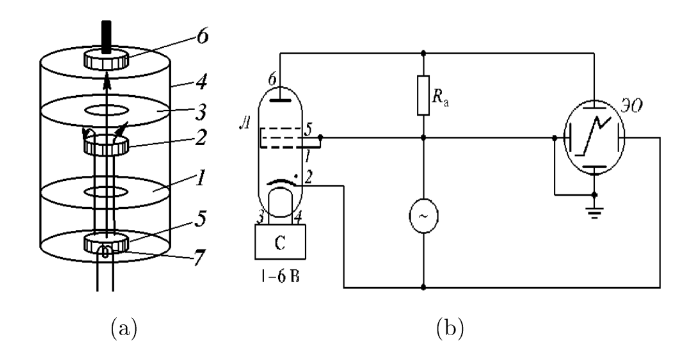
\includegraphics[width=14cm]{5.1.3-1}
		\caption{Экспериментальная установка}
	\end{center}
\end{figure}
	
	Схема экспериментальной установки, изображённая на рис.1b в нашей работе конструктивно осуществлена следующим образом. Лампа-тиратрон ТГ3-01/1.3Б, заполненная инертным газом, расположена непосредственно на корпусе блока источника питания (БИП). Напряжение к электродам лампы подаётся от источников питания, находящихся в корпусе прибора. Регулировка напряжения и выбор режима работы установки производится при помощи ручек управления, выведенных на лицевую панель БИП.
	



\section{Результаты измерений и обработка данных}

\subsection{Динамический метод}

\begin{figure}[H]
\begin{minipage}[h]{0.45\linewidth}
\center{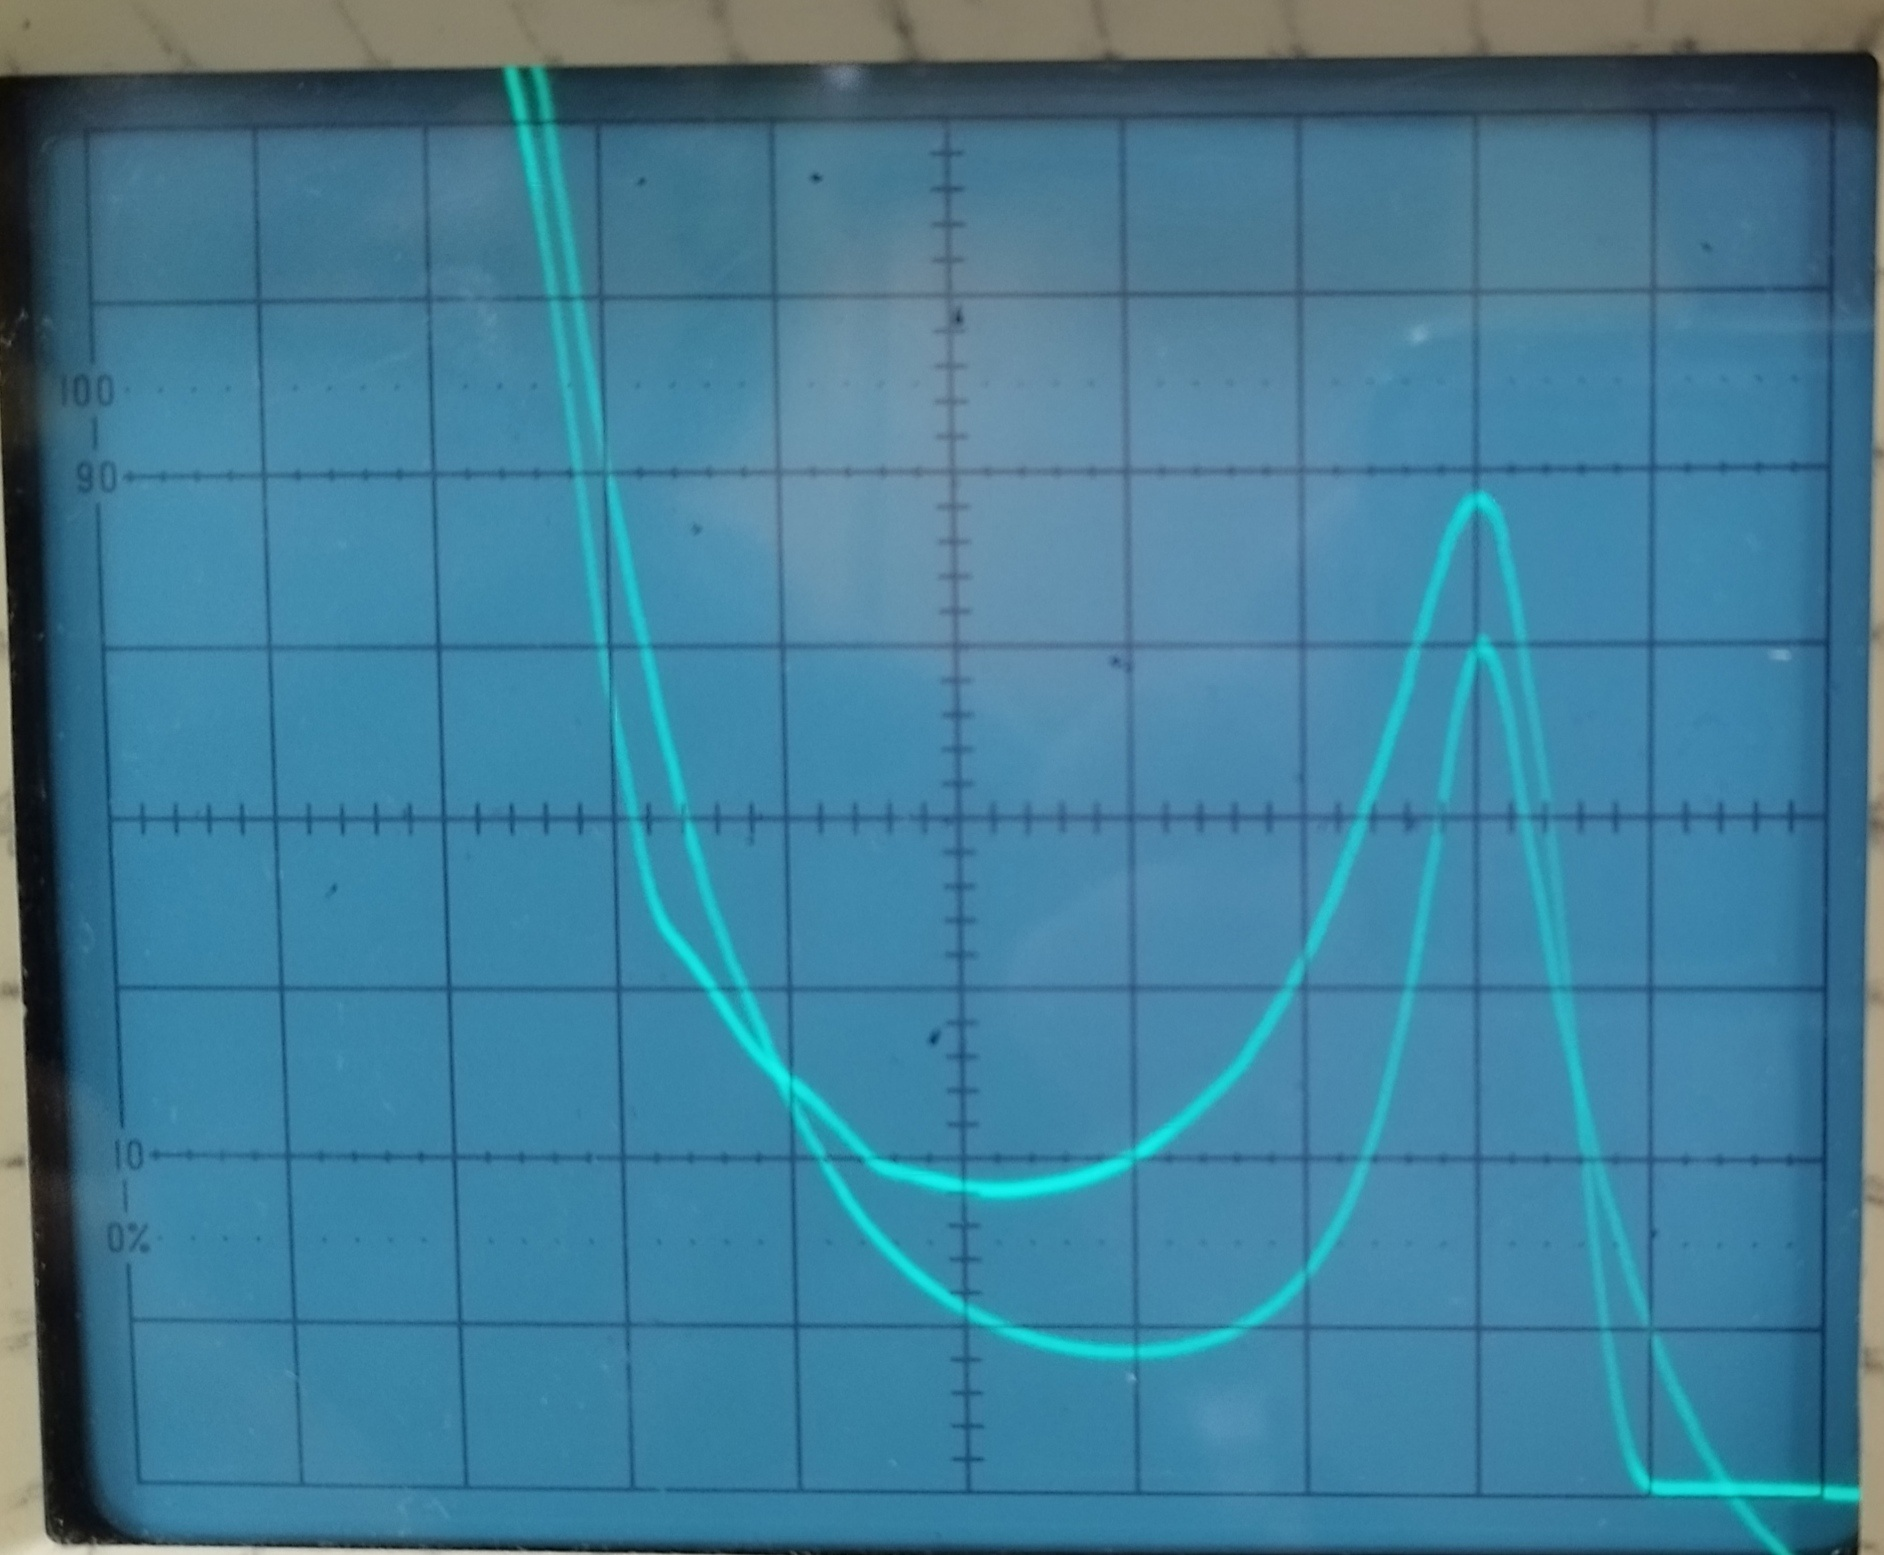
\includegraphics[width=1\linewidth]{5.1.3-2}} $V_\text{накала} = 2,93B$ \\
\end{minipage}
\hfill
\begin{minipage}[h]{0.45\linewidth}
\center{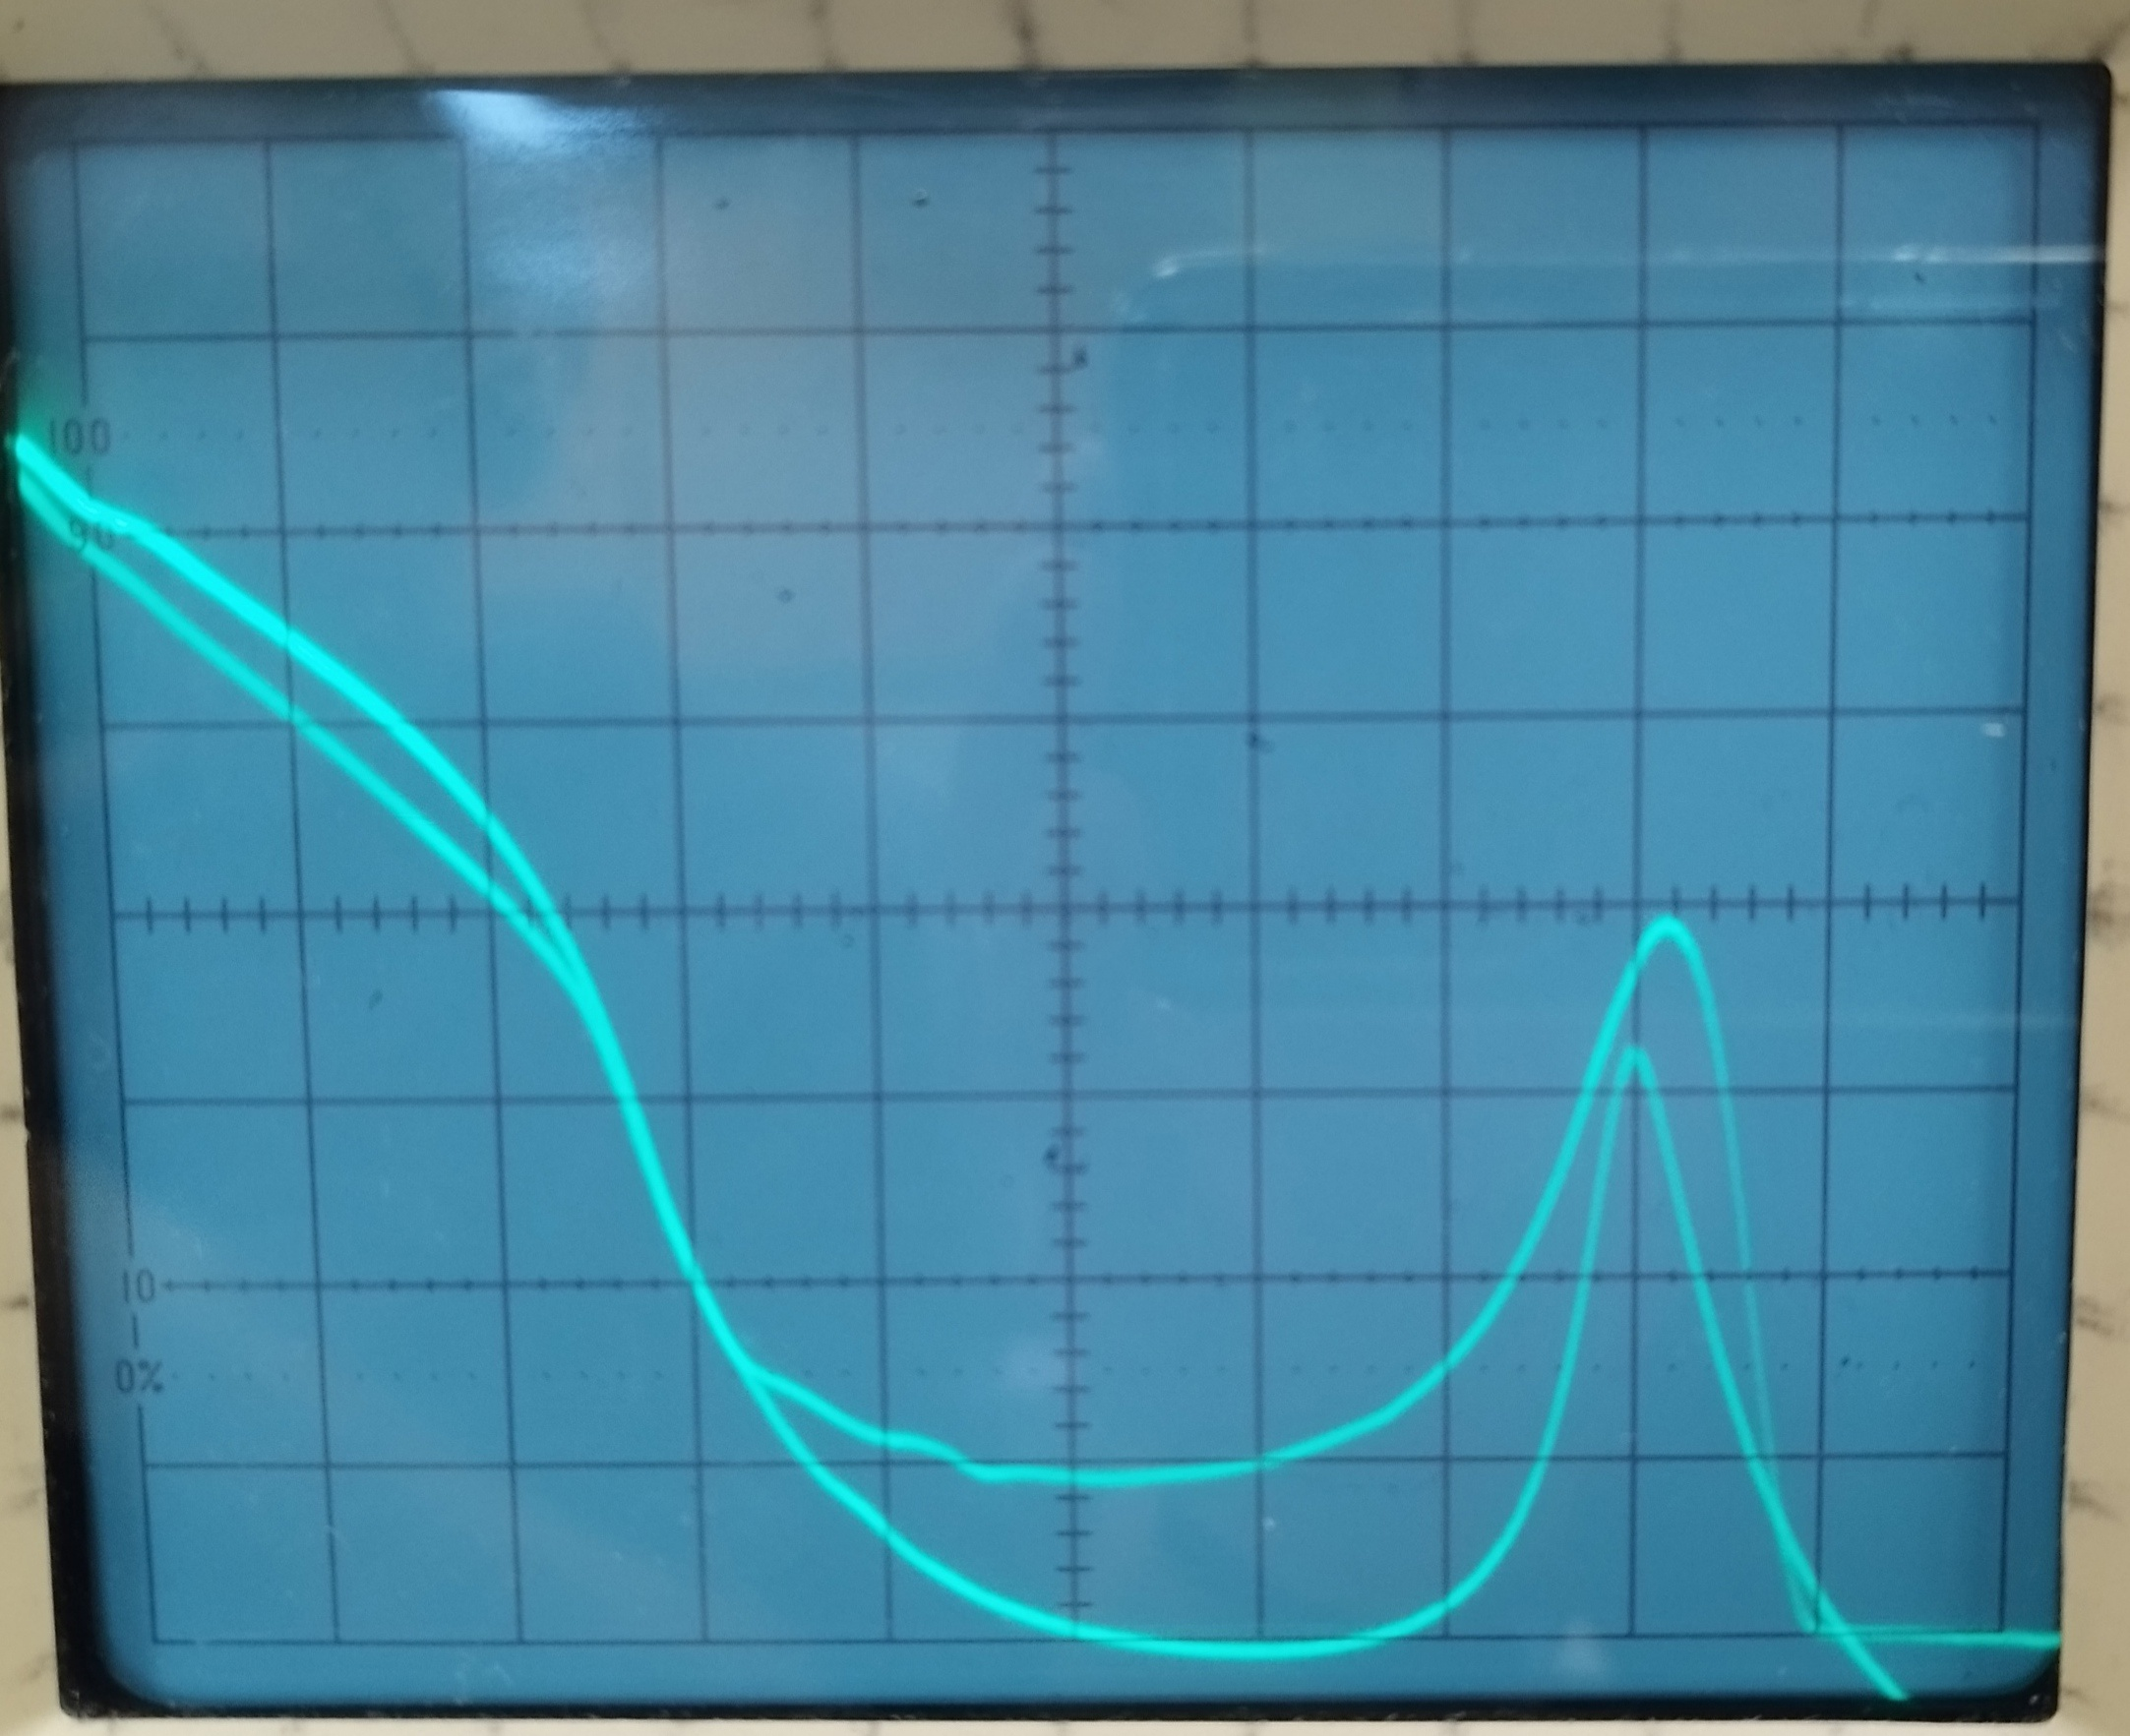
\includegraphics[width=1\linewidth]{5.1.3-3}} \\ $V_\text{накала} = 2,56B$
\end{minipage}
\end{figure}

Зная цену деления на экране осциллографа, определим энергию первого максимума, минимума, а также энергию ионизации (она примерно равна напряжению пробоя).
\hfill \break

\begin{center}
\begin{tabular}{|c|c|c|c|}
 \hline 
 $V_\text{накала}$, В  & $E_{max}$, В & $E_{min}$, B & $U_\text{ион}$, B \\ 
 \hline 
 2.93 & 2.0. $\pm$ 0.2 & 7.2 $\pm$ 0.2 & 11.6 $\pm$ 0.4 \\ 
 \hline 
 2.56  & 1.6 $\pm$ 0.2 & 8.0 $\pm$ 0.2 & 11.2 $\pm$ 0.4 \\ 
 \hline 
 \end{tabular}  
\end{center}

По формулам (3) и (4) определим размеры атома ксенона и глубину его потенциальной ямы

Погрешность l и $U_0$ оценим следующим образом:
\hfill \break

\begin{large}
$\sigma_l = l \cdot \frac{1}{2}\sigma_{E_1 - E_2} = l \cdot \frac{1}{2} \frac{\sigma_{E_1} + \sigma_{E_2}}{E_1 - E_2} $

$\sigma_{U_0} = \frac{4}{5}\sigma_{E_2} + \frac{9}{5}\sigma_{E_1}$

\begin{center}
$l = (290 \pm 30) \cdot 10^{-12} $ м 

$U_0 = (2.8 \pm 0.4)$ эВ
\end{center}

\end{large}

\begin{figure}[H]
\begin{minipage}[h]{0.45\linewidth}
\center{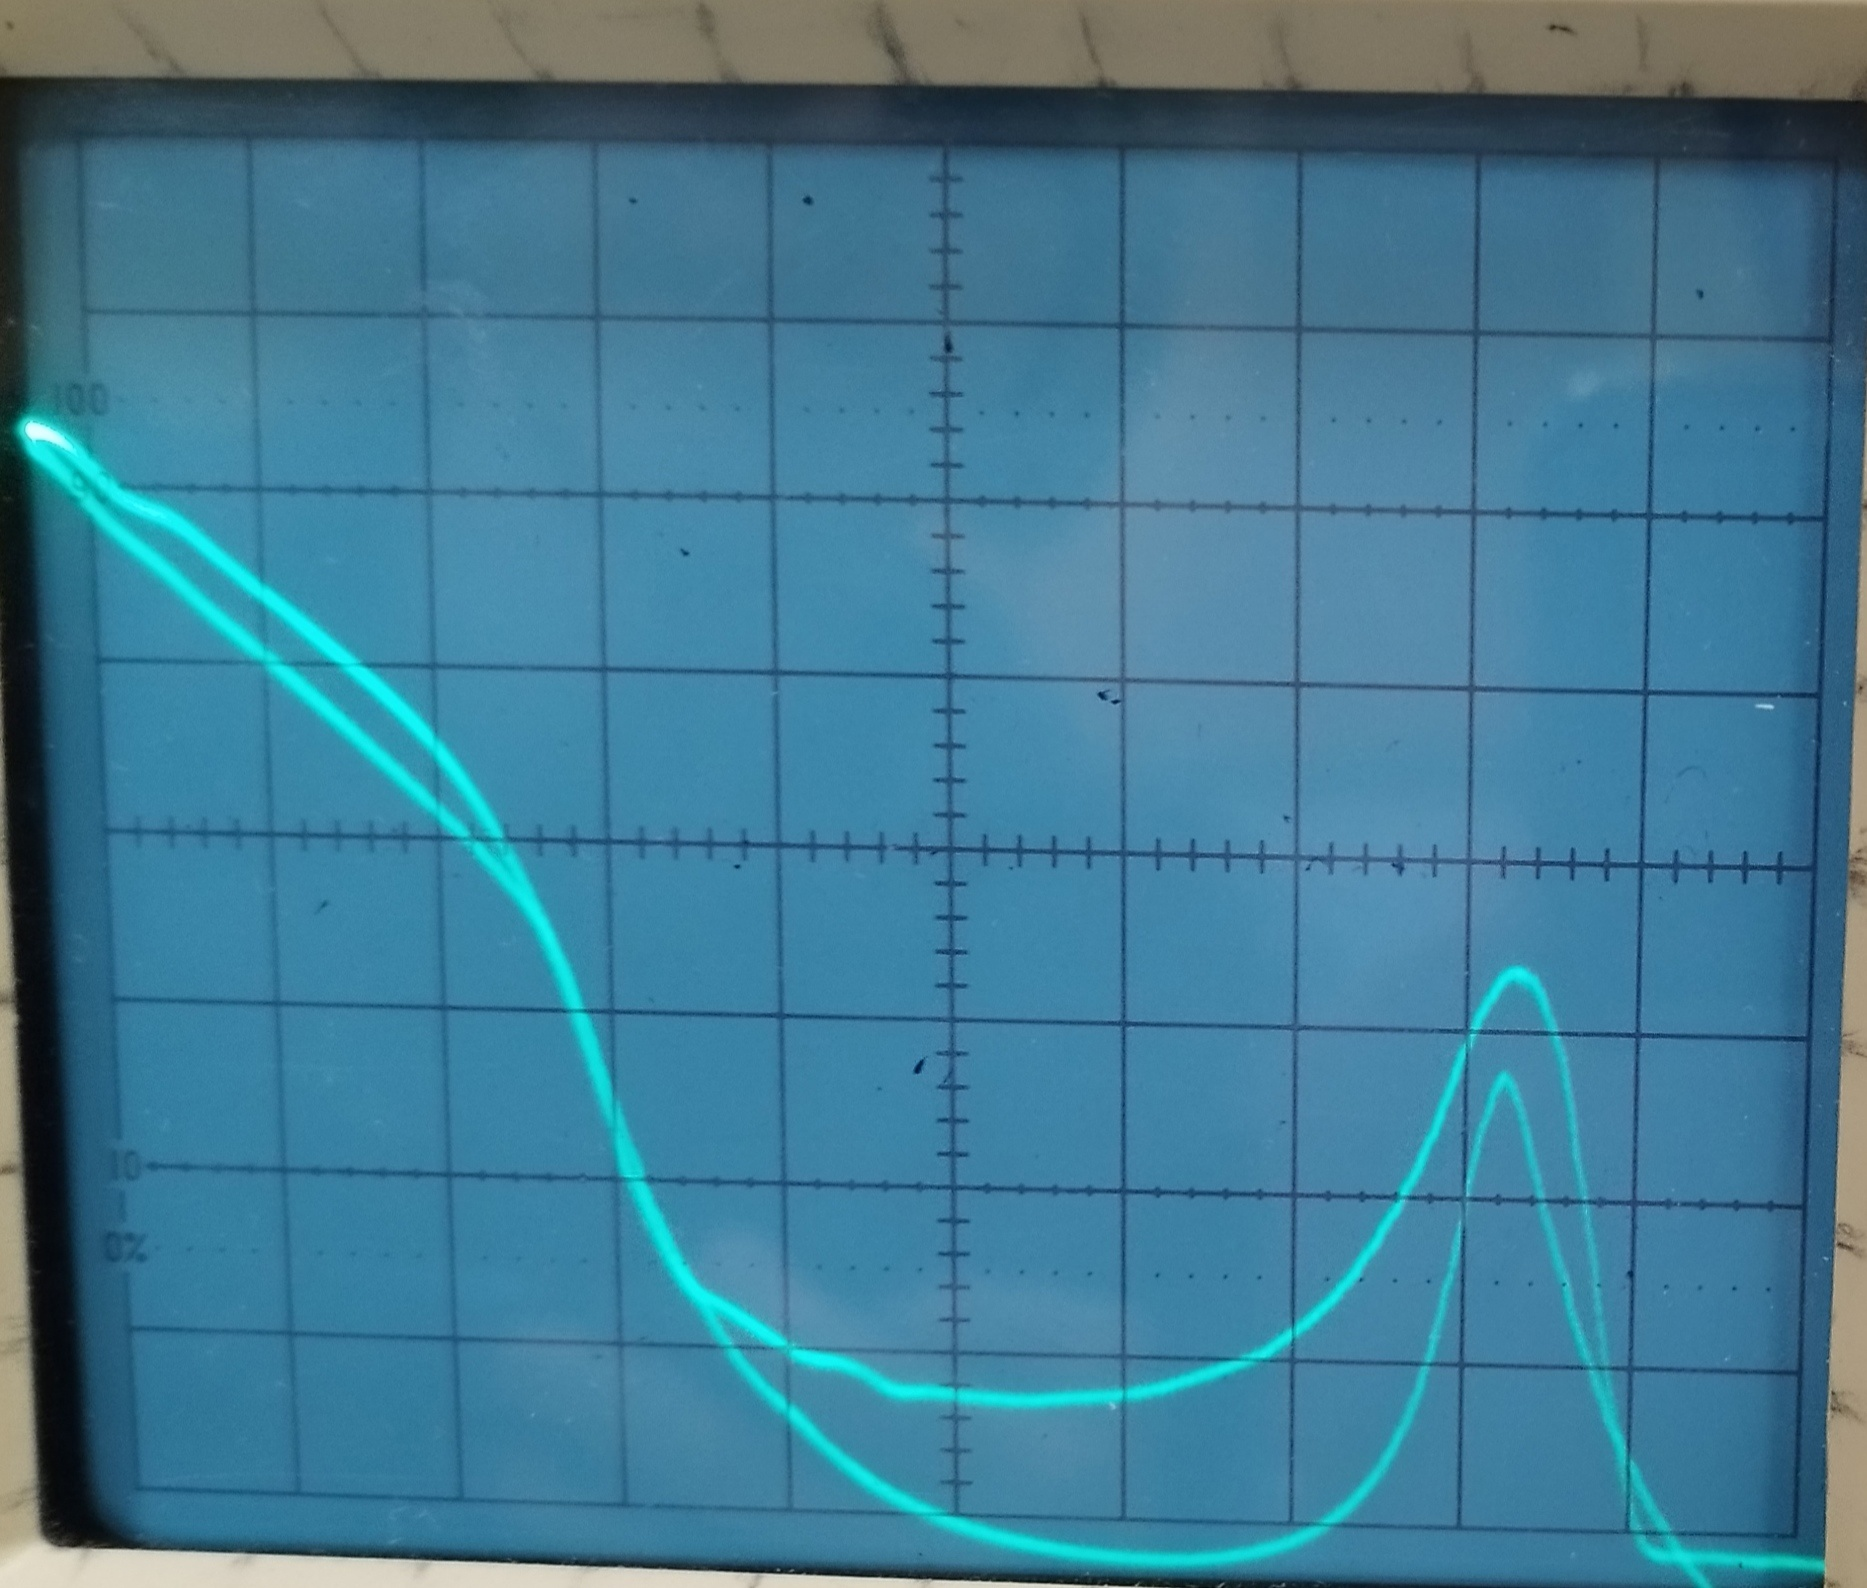
\includegraphics[width=1\linewidth]{5.1.3-4}} Магнит сверху \\
\end{minipage}
\hfill
\begin{minipage}[h]{0.45\linewidth}
\center{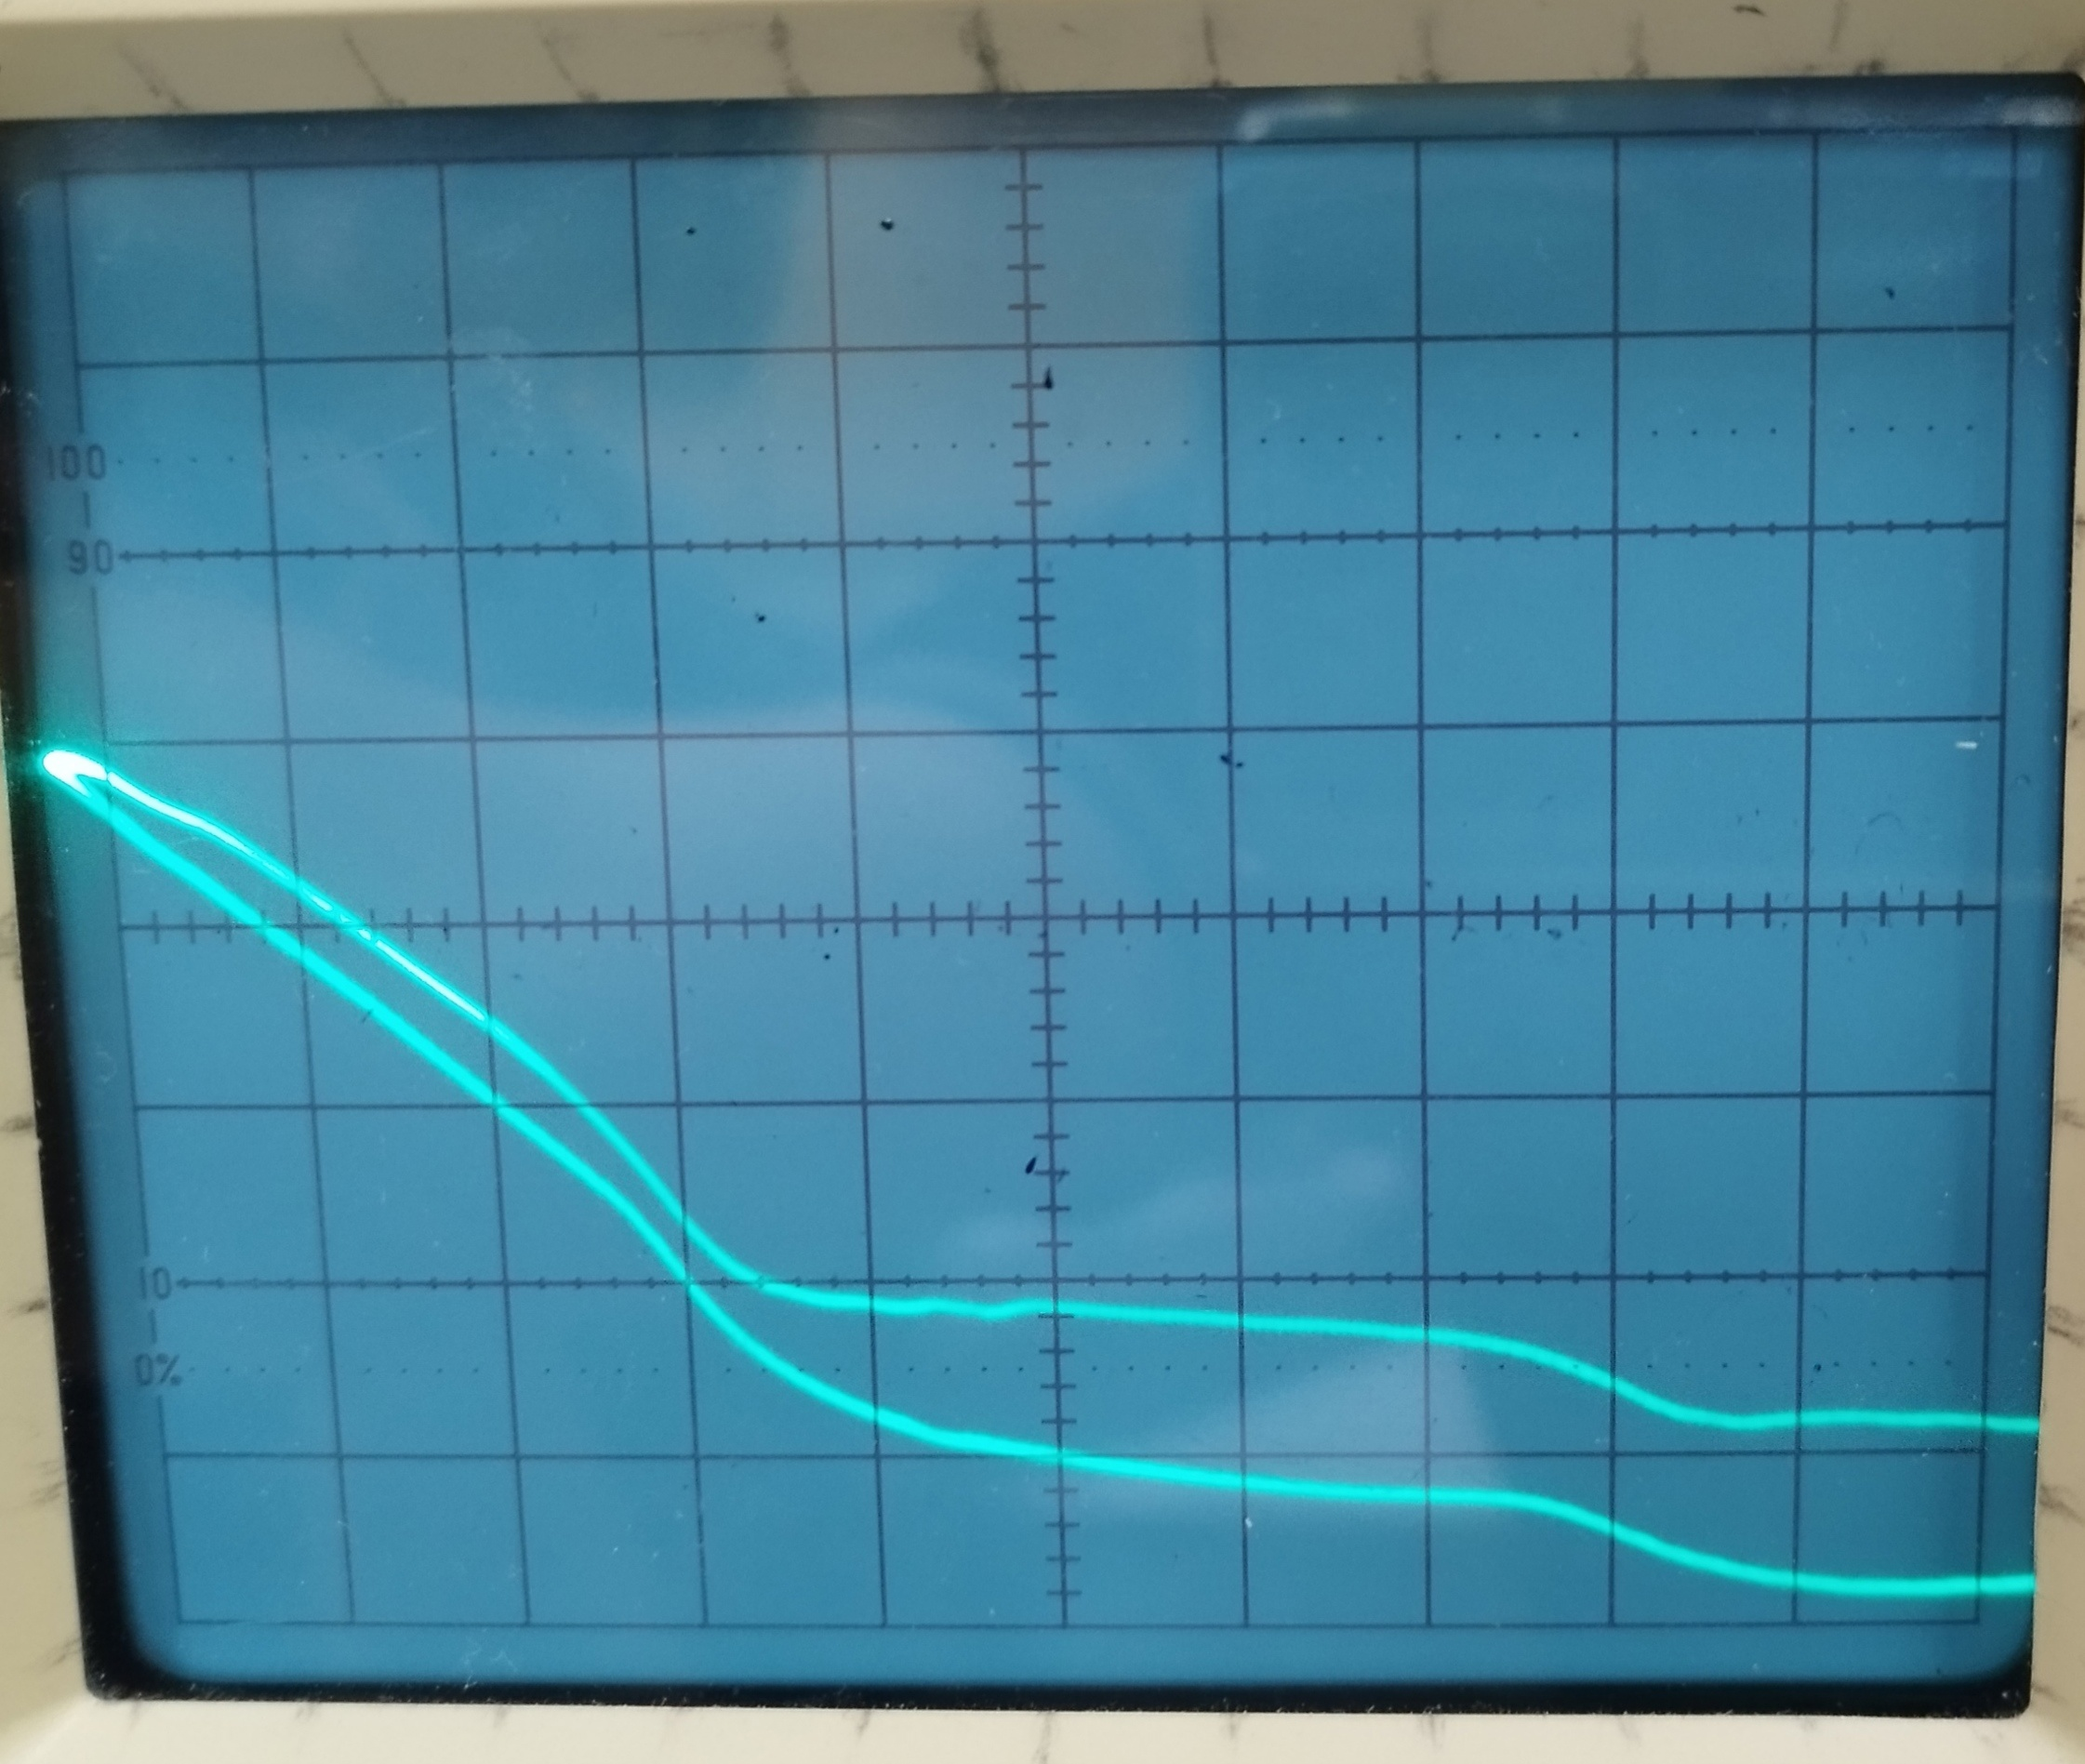
\includegraphics[width=1\linewidth]{5.1.3-5}} \\ Магнит сбоку
\end{minipage}
\end{figure}

\subsection{Статический метод}

Измерим зависимость анодного тока $I_a$ от напряжения тиратрона U. Анодный ток, ввиду отсутствия возможности измерить его напрямую, пересчитаем из напряжения на соответственном сопротивлении $R_a$ = 100 кОм

\begin{center}
U накала = 2,560 В
\begin{tabular}{|c|c|c|c|c|c|c|c|c|c|c|c|}
\hline 
U, В & 0,157 & 0,922 & 1,154 & 1,212 & 1,397 & 1,465 & 1,569 & 1,759 & 1,846 & 1,980 & 2,100 \\
\hline 
$U_a$, мВ & 0,08 & 13,72 & 60,10 & 77,36 & 126,92 & 140,40 & 158,60 & 167,40 & 168,77 & 150,45 & 143,50  \\ 
\hline 
$I_a$, мкА & 0,0008 & 0,137 & 0,601 & 0,774 & 1,269 & 1,404 & 1,586 & 1,674 & 1,688 & 1,505 & 1,435 \\ 
\hline 
U, В& 2,293 & 2,589 & 3,050 & 4,035 & 5,098 & 6,072 & 6,478 & 7,027 & 7,446 & 7,949 & 8,460  \\ 
\hline
$U_a$, мВ & 114,55 & 88,02 & 61,69 & 37,40 & 28,48 & 25,28 & 24,70 & 24,59 & 24,77 & 25,62 & 27,18  \\
\hline
$I_a$, мкА & 1,146 & 0,880 & 0,617 & 0,374 & 0,285 & 0,253 & 0,247 & 0,246 & 0,248 & 0,256 & 0,271  \\
\hline
U, B & 9,529 & 10,561 & 11,561 & & & & & & & &\\
\hline
$U_a$, мВ & 32,61 & 43,29 & 55,92 & & & & & & & & \\
\hline
$I_a$, мкА & 0,326 & 0,433 & 0,559 & & & & & & & & \\
\hline
\end{tabular} 
\end{center}

\begin{center}
U накала = 2,930 В
\begin{tabular}{|c|c|c|c|c|c|c|c|c|c|c|c|}
\hline 
U, В & 0,036 & 0,505 & 1,022 & 1,161 & 1.239 & 1,322 & 1.450 & 1,528 & 1,683 & 1,765 & 2.089 \\
\hline 
$U_a$, мВ & 0,11 & 0.85 & 62.42 & 104.63 & 130.38 & 147,67 & 176,11 & 128,28 & 189,95 & 190,20 & 171.43  \\ 
\hline 
$I_a$, мкА & 0.0011 & 0,0085 & 0,624 & 1,046 & 1,304 & 1,477 & 1,761 & 1,283 & 1,896 & 1,902 & 1,714 \\ 
\hline 
U, В& 2.180 & 2,565 & 3,049 & 3,559 & 4,093 & 4,692 & 5,282 & 6,133 & 6,853 & 7,422 & 7,954  \\ 
\hline
$U_a$, мВ & 166.18 & 138.55 & 115.77 & 100.41 & 89.76 & 82.55 & 79.00 & 78.64 & 81.93 & 86.70 & 93.26  \\
\hline
$I_a$, мкА & 1,662 & 1,386 & 1,158 & 1.004 & 0,898 & 0,826 & 0,790 & 0,786 & 0,819 & 0,867 & 0,933  \\
\hline
U, B & 8.553 & 9.031 & 9.536 & 10.064 & 10.520 & & & & & &\\
\hline
$U_a$, мВ & 103.53 & 114.07 & 124.93 & 154.46 & 170.62 & & & & & & \\
\hline
$I_a$, мкА & 1.035 & 1.141 & 1.249 & 1.545 & 1.706 & & & & & & \\
\hline
\end{tabular} 
\end{center}

\begin{figure}[H]
\begin{minipage}[h]{0.49\linewidth}
\center{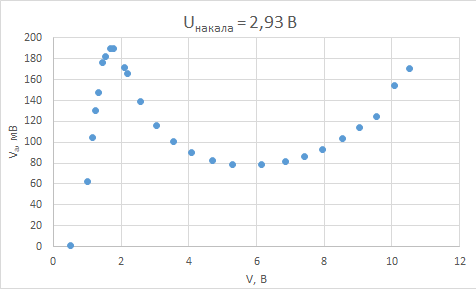
\includegraphics[width=1\linewidth]{5.1.3-6}} \\
\end{minipage}
\hfill
\begin{minipage}[h]{0.49\linewidth}
\center{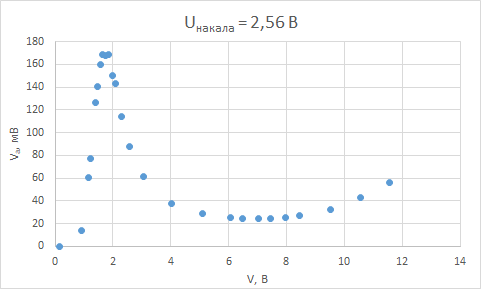
\includegraphics[width=1\linewidth]{5.1.3-7}} \\ 
\end{minipage}
\end{figure}

\begin{center}
\begin{tabular}{|c|c|c|}
 \hline 
 $V_\text{накала}$, В  & $E_{max}$, В & $E_{min}$, B  \\ 
 \hline 
 2.93 & 1.8 $\pm$ 0.2 & 6.1 $\pm$ 0.2 \\ 
 \hline 
 2.56  & 1.9 $\pm$ 0.2 & 7.0 $\pm$ 0.2 \\ 
 \hline 
 \end{tabular}  
\end{center}

Аналогично динамическому методу, рассчитаем размер атома ксенона и глубину его потенциальной ямы и их погрешности

\begin{large}
$l = (320 \pm 30) \cdot 10^{-12}$ м

$U_0 = (1.9 \pm 0.3)$ эВ
\end{large}

Оценим значения максимумов высших порядков (2-го и 3-го). Из (*) получим:
\begin{equation}
E^{max}_m = (E_1 + U_0)m^2 - U_0
\end{equation}

Таким образом,
\begin{center}
\begin{large}
$E_2^{max} \simeq 14.3$ В \;\;\;\;\;\;\;\; $E_3^{max} \simeq 35.2$ В
\end{large}
\end{center}

Данные максимумы мы не наблюдаем, т.к. они находятся дальше точки пробоя.

Построим графики вероятности рассеяния электронов. Для этого воспользуемся (5), приняв C = 1, ток катода $I_0$ за $I_a^{max}$, "перенеся" эту поправку в C.

\begin{figure}[H]
\begin{minipage}[h]{0.49\linewidth}
\center{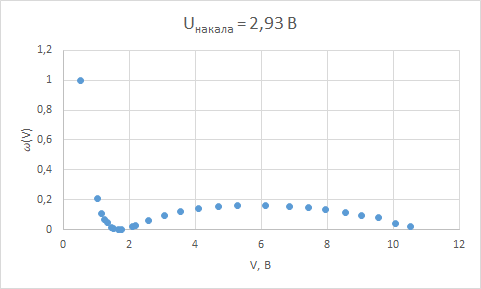
\includegraphics[width=1\linewidth]{5.1.3-8}} \\
\end{minipage}
\hfill
\begin{minipage}[h]{0.49\linewidth}
\center{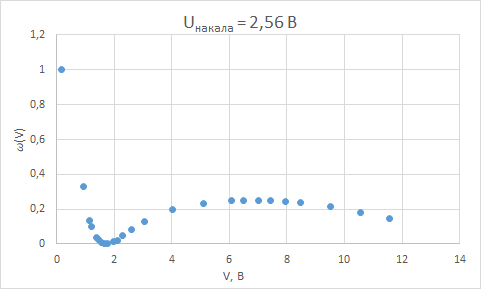
\includegraphics[width=1\linewidth]{5.1.3-9}} \\ 
\end{minipage}
\end{figure}


\section{Обсуждение результатов и выводы}
	В ходе работы провели эксперимент по исследованию эффекта Рамзауэра. В ходе него мы:

	1. Подтвердили, что газ, заполняющий тиратрон, действительно является ксеноном
	
	2. Оценили характерный размер атома и глубину потенциальной ямы двумя способами (динамическим и статическим) и получили:
\begin{center}
\begin{large}

$l^{din } \simeq 290 \cdot 10^{-12}$ м \;\;\;\;\;\;\;\; $l^{stat} \simeq 320 \cdot 10^{-12}$ м

$U_0^{din} \simeq 2,8$ эВ \;\;\;\;\;\;\;\; $U_0^{stat} \simeq 1,9$ эВ

\end{large}
\end{center}	

	3. Подтвердили, что магнитное поле обостряет эффект Рамзауэра, а при смене полярности, наоборот, сглаживает
	
	4. Нашли значения 2 и 3 максимумов, которые нельзя наблюдать так как превышается энергия пробоя.
	
	5.Получили характерный вид зависимости вероятности рассеяния электронов от катодно-анодного напряжения


\end{document}